% !TeX root = ../thesis.tex

\chapter{针对处理器微架构的攻击}{Attacks on Processor Microarchitectures}
本章将基于中科院计算所的香山高性能开源RISC-V处理器,利用处理器中的乱序执行
机制和缓存侧信道,实现一种以读取同一地址空间中存储器上任意地址内的数据为目的
的攻击方案。这种攻击方案最早在2018年初被\citet{kocher_spectre_2019}发现,
命名为Spectre(幽灵)漏洞,并在Intel Skylake及Kaby Lake微架构上得到了验证。
本研究将在香山处理器的雁栖湖微架构上实现使用与Spectre相同原理的攻击实例。


\section{高性能处理器设计理念}{High-Performance Processor Design Philosophy}
处理器设计中最主要的性能指标是单位时间内可以执行的指令数量。由于目前主流的数字
设计多采用同步设计方案(寄存器对同一个时钟边沿敏感),所以单位时间内可以执行的
指令数量就可以通过单位时间内的处理器时钟周期数量(也就是处理器的时钟频率)和每
个处理器时钟周期内可执行的指令数量(Instruction Per Cycle, IPC)相乘得到,所
以,处理器的性能与其主频和IPC都成正比,如公式\ref{eq:perf}所示。
\begin{equation}
    Performance \propto Frequency \times IPC \label{eq:perf}
\end{equation}

可见,要想提高处理器的性能,就要分别提高主频和IPC。

为了提升处理器的主频,工程师们进行了不懈的努力。处理器自上世纪70年代初进入集成
电路时代后,最初处理器的主频提升主要来自于集成电路制造工艺的优化:随着新工艺的
产生,半导体器件的漏电流及负载电容都有减小,器件间的线延迟也在减小,从而使处理
器主频不断提升:1974年,最早的个人电脑Altair 8800中使用的Intel 8080 CPU的主
频为2MHz;1992年,HP公司的PA-7100和DEC公司的Alpha 21064处理器主频突破了100MHz;
2000年,AMD公司的Athlon处理器主频达到1GHz;2002年,Intel公司的Pentium 4处理
器主频达到3GHz\cite{enwiki:clock}。

但半导体器件的动态功耗是由公式\ref{eq:pwr}决定的:
\begin{equation}
    P \propto f C V^2 \label{eq:pwr}
\end{equation}

其中$P$为功率,其主要表现形式为热能;$f$为工作频率,在处理器中即为主频;$C$为
电容,由制造工艺决定;$V$为工作电压。随着半导体制程不断下降,处理器的集成度在
升高,即单位面积内的半导体器件数量在上升,也意味着处理器的功率密度的提升。随着
越来越多的产生热量的器件集中在更小的面积内,如何控制处理器的温度以避免高温损坏
半导体器件就成了一项严峻的挑战。目前的散热技术只允许在处理器晶粒大小的面积上产
生数百瓦特的热功率,所以公式中$P$项无法有效提升。公式中的$C$项与半导体制程成
反比,但随着摩尔定律的放缓,半导体制造的特征尺寸无法快速缩减,导致电容也无法大
幅降低。而公式中的另一项$V$,受到半导体器件阈值电压的限制,目前已经降无可降。
由于上述种种限制,处理器的主频难以继续提升,这就是所谓的功耗墙。

回到公式\ref{eq:perf}中,在处理器的频率无法得到有效提高的情况下,要想提高处理
器的性能,就只能以提高处理器的IPC作为切入点。

早期的处理器设计中,每条指令都需要多个周期才能完成,例如1976年MOS Technology
公司生产的6502处理器,指令需要消耗2至7个时钟周期来完成\cite{6502manual},
每个时钟周期只有一个执行部件(如读取指令、指令译码或算术运算)会在状态机的控制下被启用。对于
这类多周期处理器,其IPC远小于1。随着计算机体系结构研究的发展,尤其是1980年之后
RISC(Reduced Instruction Set Computer,精简指令集计算机)的出现,将执行一条
指令中不同操作的执行部件以流水线的形式安排,流水级间用寄存器隔开,就可以让处于不同
执行阶段(Stage)的、正在使用不同执行部件的指令“重叠”在一起。这种流水线式的微
架构,使得处理器的IPC不断逼近1,但仍无法超过1(在一个时钟周期内执行多条指令)。
使用上述两种IPC小于1的方案设计的处理器被统称为标量处理器(Scalar Processor)。

为了追求更高的性能,就要继续想方设法提高处理器的IPC,并使之大于1,也就是处理器
需要在一个时钟周期内执行多条指令。在只有一套执行部件的处理器中,在一个时钟周期
内执行多条指令是无法实现的。但通过在流水线方案的基础上设计多套执行部件,每一个
流水级中就可以容纳与执行部件数量相当的指令。对于有$N(N = 2,3,4,\cdots)$套执行部件的处理器,每个
时钟周期最多可以提交$N$条指令,这里的$N$也被称为发射宽度。也就是在最佳情况下,使用这种方案的处理器的IPC为
$N$。使用这种IPC可以大于1方案设计的处理器被称为超标量处理器(Super-scalar Processor)。
由于这种方案在性能上的显著优势,现代高性能处理器几乎全部采用超标量设计方案。

多周期、流水线与超标量处理器中指令的执行流程如图\ref{fig:exec-cmp}所示。

\begin{figure}[ht]
	\centering
	\includegraphics[scale=1, page=2]{figs/figs.pdf}
	\caption{多周期、流水线与超标量处理器指令执行示意}
	\label{fig:exec-cmp}
\end{figure}

对于$N$发射超标量处理器,要想使IPC尽可能接近$N$,需要在每个时钟周期向执行部件
提供合适的指令(Issue,发射),避免执行部件空转。然而在每个时钟周期都选择$N$条可以并行
执行的指令并不容易,这是因为指令间往往存在依赖关系,相互间存在依赖关系的指令无法
并行执行。指令间的依赖关系主要分为两种:
数据依赖和控制流依赖。数据依赖是指后续指令的源操作数是前序指令的目标操作数的情况,
常见于算术运算指令间或存储器访问指令与算术运算指令间。控制依赖是指分支指令后的指令
是否执行取决于分支条件判断结果的情况。

要避免数据依赖影响指令的发射,可以通过调整指令的顺序,从后续指令流中选取尽可能多
相互之间无依赖关系的指令进行发射,这种操作被称为指令的动态调度(Dynamic Scheduling)。
但调整指令执行顺序会打破指令集中规定的指令流顺序执行抽象,这就需要使用一些手段使得
指令的执行结果变得对程序员可见(指令对体系结构状态的修改,也就是提交)按照程序指令
流顺序发生,常见的此类手段为重排序缓冲区(Reorder Buffer)。这种在处理器运行过程
中动态调整程序指令顺序的技术被称为乱序执行(Out-of-Order Execution)。

而为了减小指令间的控制流依赖对指令的发射造成负面影响,可以在指令流遇到分支时预测
指令流跳转的方向以及跳转目标,这样不必等待分支条件计算,也就不会导致指令流的中断。
这种手段行之有效的原因是:分支指令的条件判断结果在统计学上存在一定的规律,并且不
同的分支指令判断结果的历史间也存在着一定的联系。目前成熟的分支预测器在绝大部分情
况下对分支跳转方向的预测正确率可达到95\%以上。此外,处理器在沿着猜测的分支方向
执行时,也会保留分支点状态的快照,这样即使分支条件的计算结果证明先前的猜测是错误的,
处理器也可以很快将状态恢复到分支点,并继续沿着正确的分支方向执行。这种在得到分支
条件计算结果前沿着预测的跳转方向继续执行的技术被称为预测式执行(Speculative Execution)。

运用上述乱序执行以及预测式执行的机制,现代高性能处理器的IPC已经可以达到3这样的
较高水平\cite{zhao2020sonicboom},并且处理器执行流水线的性能已经不是整个处理
器系统的瓶颈。俗话说“巧妇难为无米之炊”,处理器执行流水线所需的指令和数据都存储
在动态随机存储器(Dynamic Random Access Memory,DRAM)中,但DRAM的访问延迟
多为数百纳秒,近千倍于处理器主频。这意味着如果不采取措施,处理器每次从DRAM中
读取指令和数据时,都要等待近千个时钟周期。为了解决DRAM延迟与处理器速度不匹配的
问题,现代处理器的存储器子系统采用分级的架构:越靠近处理器执行流水线的存储器
容量越小,但延迟越低,例如可以将与流水线工作在同一频率的体系结构寄存器视为一级
“缓存”,其容量最小,但延迟为零。并在DRAM到寄存器间插入多级(一般为2至3级)高速
缓存(Cache)。采取分级存储器子系统设计方案的原因主要有两个:
一是受到当前半导体器件工艺的限制,存储器的容量和延迟成反比,即越小越快,越大越慢;
二是程序访问存储器(包括指令和数据)的模式具有时间局部性和空间局部性的特点,也
就是程序近期访问的存储器地址也可能在将来再次被访问,并且这一地址附近的地址也可能
在将来被访问到。图\ref{fig:mem-heir}给出了一款处理器(Intel Core i7-10875H)
的存储器子系统示意图,图中注明了各级存储器的容量及延迟。

\begin{figure}[ht]
	\centering
	\includegraphics[scale=1, page=3]{figs/figs.pdf}
	\caption{存储器子系统分级示意}
	\label{fig:mem-heir}
\end{figure}

综上所述,现代高性能处理器主要采用的设计方案是:具有乱序执行以及预测式执行特点的
超标量流水线,和分级的存储器子系统。


\section{香山处理器南湖微架构简介}{Introduction to Nanhu Microarchitecture of Xiangshan Processor}
香山处理器是2019年在中国科学院支持下,由中国科学院计算技术研究所牵头发起的高性能开源
RISC-V处理器项目。南湖是香山处理器第二版微架构代号,支持RV64GCBK指令集,已在2022年3月
完成RTL代码冻结,正在进行后端设计验证流程并将在2022年上半年完成投片,目标是在14nm工艺
节点下频率达到2GHz。

南湖微架构的流水线分为前端和后端两个部分。前端流水线包括分支预测单元、取指单元、指令
缓冲等单元,预测式地取指。后端包括译码、重命名、重定序缓冲、保留站、整型/浮点寄存器堆、
整型/浮点运算单元、访存流水线(包括两条读取流水线,两条写入地址流水线,
两条写入数据流水线,以及独立的读取队列、写入队列和写入缓冲区等)。其微架构如图\ref{fig:nanhu-uarch}所示。

\begin{figure}[ht]
	\centering
	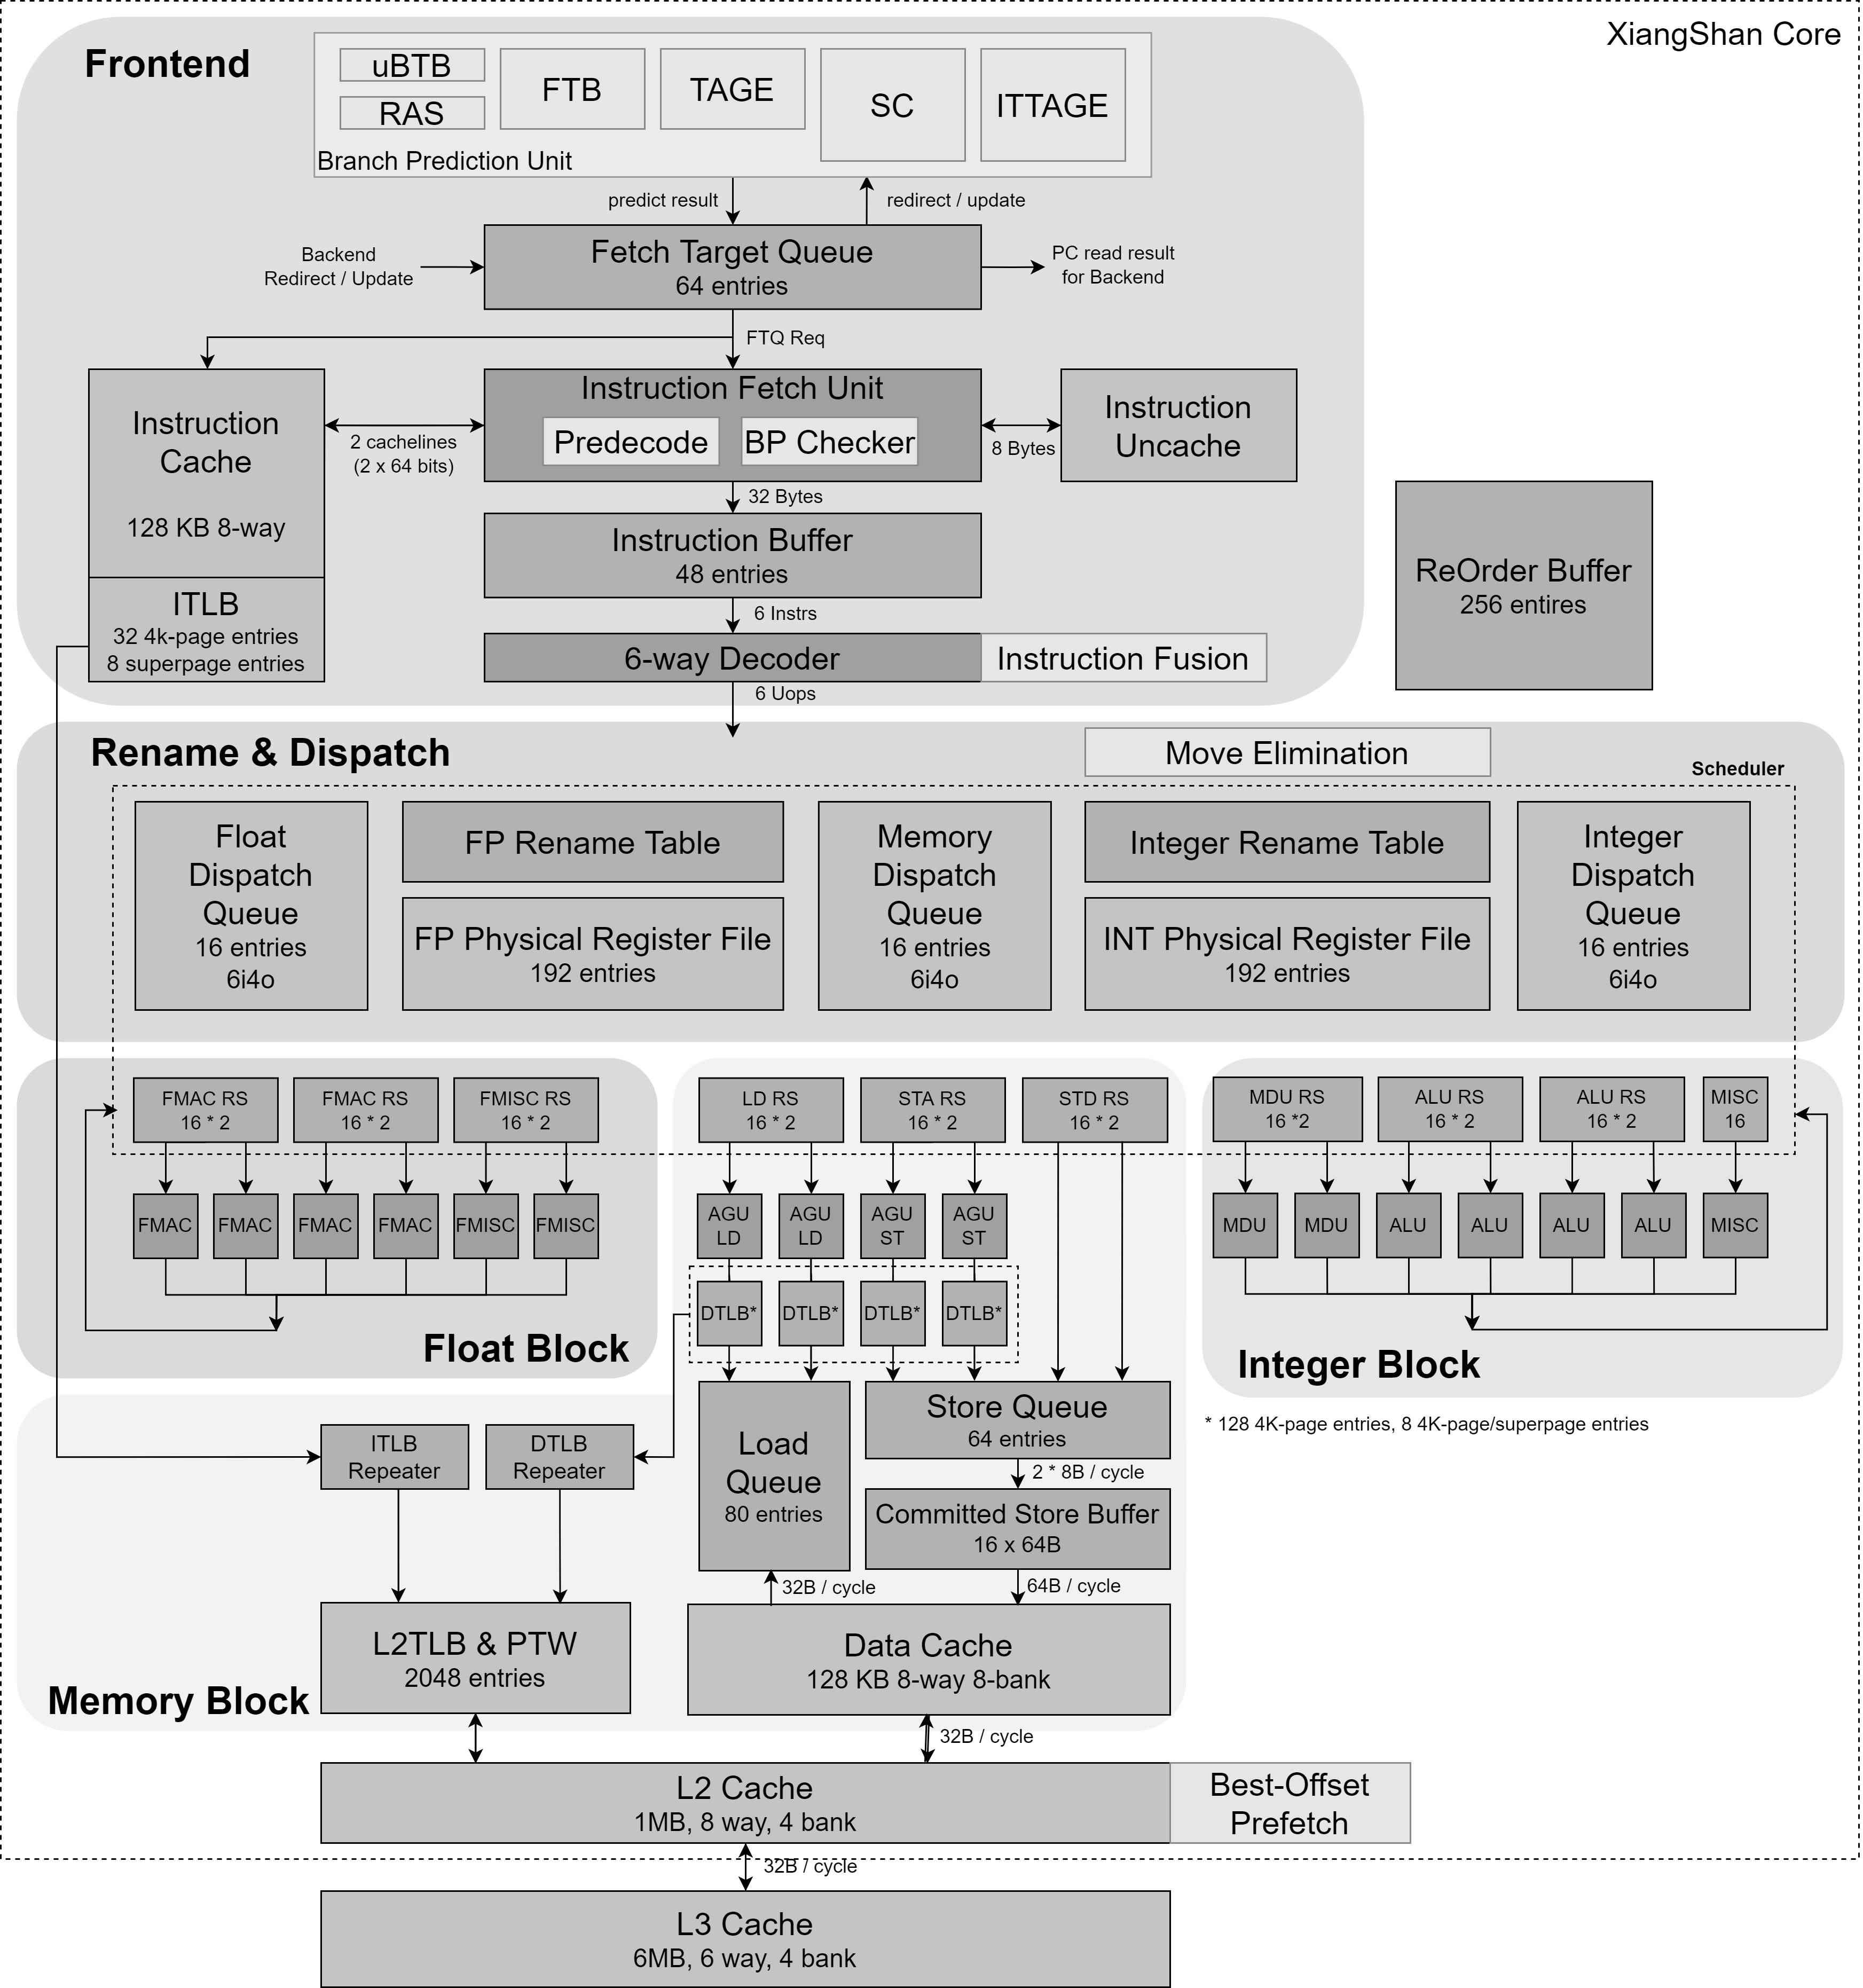
\includegraphics[width=\textwidth]{figs/nanhu.png}
	\caption{南湖微架构\cite{noauthor_openxiangshan/xiangshan:_nodate}}
	\label{fig:nanhu-uarch}
\end{figure}

由于本章展示的攻击方案围绕南湖微架构展开,本小节将对南湖微架构中与攻击方案有关的预测式
执行、乱序执行机制以及存储器子系统的设计作简单的介绍。

\clearpage

\subsection{预测式执行机制}{Speculative Execution Mechanism}
进入南湖微架构执行流水线的每一条指令的地址都是由分支预测单元(Branch Prediction Unit)提供的。
南湖微架构采取了一种分支预测和指令缓存解耦的取指架构,分支预测单元预测接下来的取指地址,
作为取指请求写入一个队列,这个队列将其发往取指单元,用于读取指令高速缓存(Instruction Cache)。

分支预测单元采用一种多级混合预测的架构,其主要组成部分包括:下一行预测器(Next Line Predictor,NLP)
和精确预测器(Accurate Predictor,APD)。其中,NLP是一个小型跳转目标缓冲区(Micro Branch Target Buffer),
用较小的存储开销提供一个无空泡的快速预测流。
APD中运用了TAGE-SC(TAgged GEometric Length Predictor with Statistical Corrector)
算法用来预测分支方向,并设计有取指地址缓冲区(Fetch Target Buffer)和返回地址栈(Return Address Stack)
用以提供跳转地址。
上述部件都将流水线的提交记录作为训练源,以实现根据历史指令流预测未来指令流的功能。

\subsection{乱序执行机制}{Out-of-Order Execution Mechanism}
在指令的发射阶段,南湖微架构使用保留站(Reservation Station)这一结构选择依赖关系已得到
满足的指令送入执行单元,以实现乱序执行。保留站内的主要存储了指令状态、指令和依赖数据。
保留站对指令进行的操作主要有:在发射阶段的入队、选择、读数据和出队等,在写回阶段的监听
以及对等待指令的唤醒等。保留站的主要模块还包括选择逻辑,用来为入队指令分配空闲表项、选择
就绪的指令进行发射。

运用上述硬件结构,可以实现以数据就绪作为指令可以执行的标准,从而指令被执行的顺序可以和
程序指令流中指令出现的顺序不同。

\subsection{存储器子系统}{Memory Subsystem}
香山处理器南湖微架构的存储器子系统可以分为核内和核外两个部分。

位于核内的存储器子系统包括执行单元中的读取、写入地址、写入数据流水线,
读取队列、写入队列和写入缓冲区,与流水线紧耦合的一级数据高速缓存(L1 Data Cache),
以及存储器管理单元(MMU,包括转译后备缓冲器TLB以及页表遍历器TLB)。

位于核外的存储器子系统主要是二级高速缓存(L2 Cache)。这一高速缓存同时具有一致性管理器(Coherence Manager)
的功能,为基于目录的非包含高速缓存(Directory-Based Non-Inclusive Cache),这意味着
在二级高速缓存内维护者一个列表,记录了目前存在于一级高速缓存中的地址(但并不同时存储这些
地址对应的数据),这允许二级高速缓存在外部接口收到一致性维护请求后,通过内部接口通知一级
高速缓存提供最新的数据并将对应缓存行(Cache Line)置为无效状态。


\section{攻击方案}{Attack Plan}
Spectre v1 Bounds Check Bypass
Flush + Reload
\somewords


\section{可行性验证}{Feasibility Verification}
\somewords
\subsection{缓存控制与检测}{Cache Manipulation and Measurement}
flush cache line
Timed read
\subsection{误导预测执行流}{Misleading Speculative Execution Stream}
Training
\subsection{香山南湖架构攻击验证}{Attack Verification on Nanhu Microarchitecture}
\somewords


\section{本章小结}{Chapter Summary}
\somewords


\newpage
